\documentclass{fisatproject}
\usepackage{graphicx}
\title{Peer2Chat - Decentralized Chat App }
\team{Dharwish Raj - FIT17CS046 \\ Adhyaksh Guhan - FIT17CS007 \\ Allen Raphael Sunny - FIT15CS015 \\ Ajay Diji - FIT17CS009}
\author{Dharwish Raj(FIT17CS046), Adhyaksh Guhan(FIT17CS007), Allen Raphael Sunny(FIT15CS015), Ajay Diji(FIT17CS009)}
\begin{document}
\maketitle

\makecert

\newpage
%\thispagestyle{plain}
\pagenumbering{roman}
\setcounter{page}{1}
\newgeometry{top=4cm,bottom=0.1cm}
\renewcommand\abstractname{ABSTRACT}
\begin{abstract}
\vspace{5cm}
A decentralised application is one that does lies outside the purview and control of a single authority. This enables the app to allow for transfer of data with complete anonimity and interruptions from third-parties. This project uses a peer-to-peer (p2p) network to enable communication between multiple parties in a decentralised fashion.
\end{abstract}


\newpage
%\thispagestyle{plain}
\renewcommand\abstractname{ACKNOWLEDGMENT}
\begin{abstract}
\vspace{5cm}
If words are considered as symbols of approval and tokens of acknowledgment , then let the words play the heralding role of expressing our gratitude. \\ \\
 \textbf{Ms. Anitha P}, Chairman, Governing Body-FISAT, who provided us with vital facilities required by the project right from the inception to completion. \\ \\
 We express our deepest appreciation towards \textbf{Dr. George Issac}, Principal ,FISAT, for providing amenities, which helped us in the fulfillment of our project. \\ \\
 \textbf{Dr. Prasad J.C} , Head of Department of Computer Science and Engineering, FISAT, guided us  and rendered his help in all phases of our project. \\ \\
 We would also like to express our gratitude to \textbf{Ms. Sruthy Suresh , Ms. Divya John}, had been a pillar of support for the successful completion of our project. \\ \\
 Last but not the least, we express our sincere gratitude to all the staffs of the Department of Computer Science  and Engineering, who helped us in the course of work. \\ \\

\vspace{1cm}
\begin{flushright}
Dharwish Raj(FIT17CS046)

Adhyaksh Guhan(FIT17CS007)

Allen Raphael Sunny(FIT15CS015)

Ajay Diji(FIT17CS009)
\end{flushright}
\end{abstract}
\newpage

\restoregeometry
\tableofcontents

\newpage
\pagestyle{fancy}


\chapter{INTRODUCTION}
\pagenumbering{arabic}
\setcounter{page}{1}
\renewcommand{\baselinestretch}{1.50}
\section{Overview}
Decentralised networks, as opposed to centralised networks, are organised in a much more distributed fashion. Each node within the network functions as a separate authority with independent decision-making power regarding how it interacts with other systems. These networks also distribute processing power and workload functions among connected servers. This creates a lack of any central power that can maintain control over the whole network and control how information flows within it. The P2P based chat app utlises this philosophy and can connect one peer to another to start a conversation in complete anonimity.

	\subsection{Peer-to-peer}
	Peer-to-peer (P2P) computing or networking is a distributed application architecture that partitions tasks or workloads between peers. Files can be shared directly between systems on the network without the need of a central server. In other words, each computer on a P2P network becomes a file server as well as a client.
	
	\begin{center}
		\begin{figure}[h]
			
			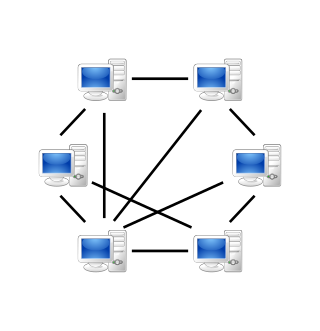
\includegraphics[width=8.2cm]{p2p.png}
			\caption{A p2p network}
			
		\end{figure}
	\end{center}
	The only requirements for a computer to join a peer-to-peer network are an Internet connection and P2P software. Common P2P software programs include Kazaa, Limewire, BearShare, Morpheus, and Acquisition. Once connected to the network, P2P software allows a user to search for files on other people's computers. Meanwhile, other users on the network can search for files on the user's computer, but typically only within a single folder that is designated to share. 
	
	\subsection{Advantages}

	\begin{itemize}
		\item \textbf{Easy of setup and maintanence}
		The network is fast and inexpensive to setup and maintain as it requires no dedicated servers since all users act as both client and server.
		
		\item \textbf{More reliable}
		The failure of a single peer in the network does not affect all other peers in the rest of the network due its decentralised nature.
		
		\item \textbf{Access to shared resources}
		The user can control their shared resources and can set any resource as accessible as long as it is in a shared folder. This negates the need of a System Administrator.
		
	\end{itemize}
	
	\begin{center}
		\begin{figure}[h]
			
			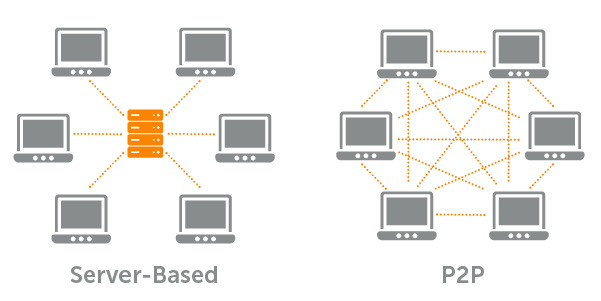
\includegraphics[scale=.75]{svp.jpg}
			\caption{Server based vs P2P}
			
		\end{figure}
	\end{center}
\newpage
	\subsection{WebRTC}

\begin{itemize}
	\item \textbf{About WebRTC}
	
	WebRTC (Web Real-Time Communication) is a free, open-source project that provides web browsers and mobile applications with real-time communication (RTC) via simple application programming interfaces (APIs). It allows audio and video communication to work inside web pages by allowing direct peer-to-peer communication, eliminating the need to install plugins or download native apps.
	
	\item \textbf{Why WebRTC over WebSockets}
		\item WebSocket is a computer communications protocol whereas WebRTC is a free open source project that enables browsers and mobile applications with communication capabilities.
		\item Though both WebSockets vs WebRTC are communication protocols, WebRTC is used for more Real-Time Applications when in comparison to WebSockets.
		\item WebRTC is designed for high-performance, high-quality communication of video, audio and arbitrary data. WebRTC apps need a service via which they can exchange network and media metadata, a process known as signaling. WebSocket, on the other hand, is designed for bi-directional communication between client and server. It is possible to stream and share audio and video over WebSocket but, the API is not robust enough like their counterpart features in WebRTC.
	

	
\end{itemize}

	\begin{center}
	\begin{figure}[h]
		
		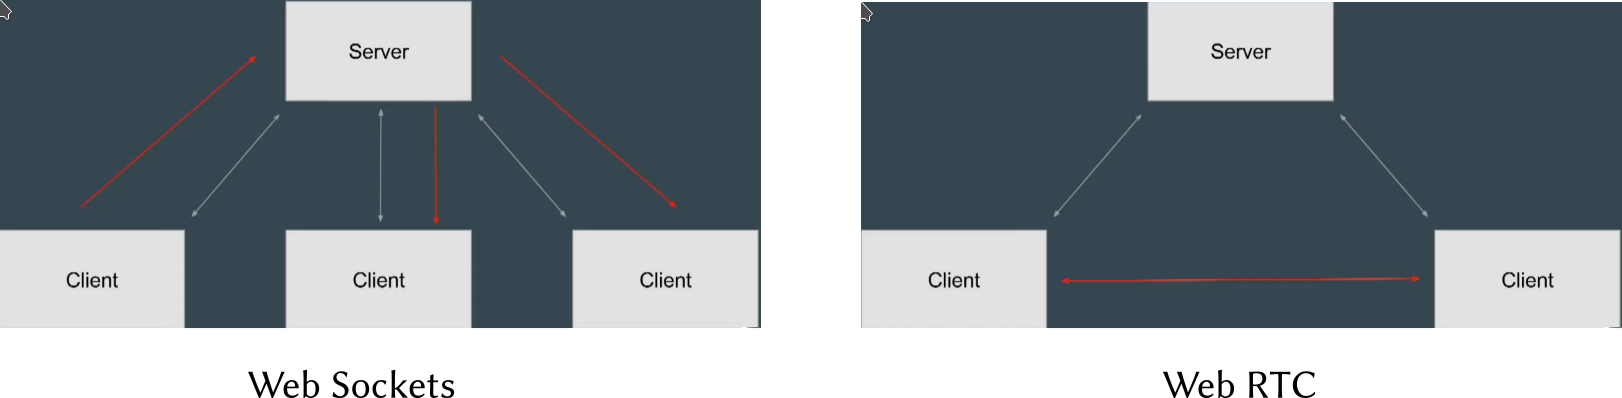
\includegraphics[scale=.37]{webrtcfig.png}
		\caption{Web Socket vs Web RTC}
		
	\end{figure}
\end{center}


\chapter{RELATED WORK}

\begin{itemize}
	\item \textbf{1. Augur}
	Augur combines decentralized networking and financial prediction markets to create powerful forecasting. It’s built upon the Ethereum blockchain. In its current guise, Augur allows you to make predictions about real-world events not limited to financial markets. The platform turns your prediction into “shares” that other users can buy or sell.
	

	\item \textbf{2. Vett.space}
	This is that game made online. It's an online multiplayer implementation of Dots-and-Boxes !
	Built with VueJS, d3.js, P2PT. Uses WebTorrent trackers for making Peer-to-Peer connections for multiplayer.
	

	\item \textbf{3. Aragon}
	
	Aragon is an ambitious decentralized management platform, also built on the Ethereum blockchain. It wants to break down the traditional barriers that restrict the creation and maintenance of organizational structures. In other words, Aragon wants to make it easier to create private Decentralized Autonomous Organizations (DAOs), along with everything you need to succeed. This means arbitration, token management and transfers, role assignments, fundraising, and much more.

	\item \textbf{4. Sia}
	
	Sia is a promising decentralized storage platform that leverages “underutilized hard drive capacity around the world,” creating a first-of-its-kind blockchain-based data storage marketplace. The platform turns those empty hard drives into cheap cloud storage that almost anyone can use. Prices are cheap, especially when compared to other major cloud storage providers.
	
	\item \textbf{5. SAFE Network}
	
	The SAFE Network uses a decentralized approach to protecting consumer data and private communication. SAFE, which stands for Secure Access For Everyone, uses peer-to-peer technology to share that computing power between connected users. This creates a secure private network, rather than relying on centralized servers.
\end{itemize}


\chapter{DESIGN and IMPLEMENTATION}

\section{Design}

Peer2Chat is implemented using following technologies : 
  \begin{itemize}
 \item A web peer2peer communicating library called p2pt which developed using WebTorrent modules 
 \item A JavaScript program that initiate Torrent trackers and accept peer list and packets passed
 \item A web application interface for above programe runs on Vue.js 
 \end{itemize}

   \subsection{How this works}
   
    	\subsubsection{Peer-to-Peer Communication}
   WebTorrent is a library which created a new kind of Torrent Trackers called \textbf{"WebSocket Trackers"}  also known as "WebTorrent Trackers". Most of the torrent clients are using this technology to share files. But web-based  clients have a limitation that it  JavaScript in browser can't directly make TCP/IP connections and communicate. To overcome this problem, we use WebRTC. WebRTC is the method by which browsers can communicate to other browsers peer to peer (P2P). WebTorrent makes use of WebRTC for sharing Torrents on web. But to establish peer2peer connection between WebRTC a signalling server is needed. To avoid that we use WebSocket trackers as the singling servers to establish communication between clients.  
   		\subsubsection{Finding Clients (Peers)}
   		We use a magnet link. The magnet link has a unique identifier for our torrent called the \textbf{Info Hash}. This ID will be unique for all torrents.
   		
   		Similarly, to implemented chat app, we use an identifier. This identifier is converted to a valid Info Hash and sent to our WebTorrent trackers who will give us a list of web peers. These web peers would be the other users also using our app.



   \vspace{1cm}
  
 
    
    \vspace{1cm}
    \subsection{User Interface}
    The front-end interface of our chat application is build using Vue.js, which will help single page navigation compared to regular HTML/CSS.
    \newpage

\section{Implementation}
    What is basically happening here is that when client load this app, Trackers will pass InfoHash to the new client which contains manget link.
    
        \vspace{0.6cm}
Announcing Trackers URL in app.js  
	\begin{lstlisting}[language=java]
	let announceURLs = [
	"wss://tracker.openwebtorrent.com",
	"wss://tracker.sloppyta.co:443/announce",
	"wss://tracker.novage.com.ua:443/announce",
	"wss://tracker.btorrent.xyz:443/announce",
	]
	if (window.location.hostname === "localhost") {
	announceURLs = ["ws://localhost:5000"]
   });
   \end{lstlisting}
           \vspace{0.6cm}
   Magnet link will help to generate peer list (connected clients) on every client, so that it will establish communication with peers (clients using WebRTC)
   
   
              \vspace{0.6cm}
              Connect to network and start discovering peers in p2pt
	 \begin{lstlisting}[language=java]
	 start () {
	 const $this = this
	 
	 this.on('peer', (peer) => {
	 var newpeer = false
	 if (!$this.peers[peer.id]) {
	 newpeer = true
	 $this.peers[peer.id] = {}
	 $this.responseWaiting[peer.id] = {}
	 }
	 
	 peer.on('connect', () => {
	 $this.peers[peer.id][peer.channelName] = peer
	 
	 if (newpeer) {
	 $this.emit('peerconnect', peer)
	 }
	 })
	    \end{lstlisting}
        \vspace{0.6cm}

    

Next we implementing function to join, send and revive data between client in App.js
         \vspace{0.6cm}
 	 \begin{lstlisting}[language=java]
 	 
 	 \end{lstlisting}


\chapter{TESTING}
The project was implemented by testing at multiple stages. First we tested whether we can find a peer using Web Trackers.
	\begin{center}
	\begin{figure}[h]
		
		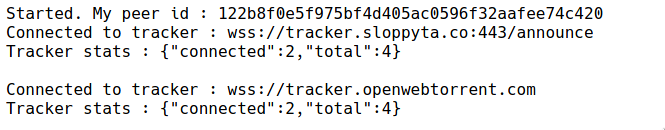
\includegraphics[scale=.37]{testpeer.png}
		\caption{Peer Find Test using Web Trackers}
		
	\end{figure}
\end{center}

Then implemented web-app using Vue.js and tested multiple client scenario, Join Chat, Sending Message and also connecting to multiple devices.
\chapter{RESULTS}


The final result of the project, after finding another peer through the tracker, connecting to them, is a two way communication and sharing of resources between the users. There was a flow of information that enabled coversation on both sides and could also read the text that was sent by them as well as from the other user. After disconnecting, the user's record of conversation could only be found on each other's computer.
\newpage
	\begin{center}
	\begin{figure}[h]
		
		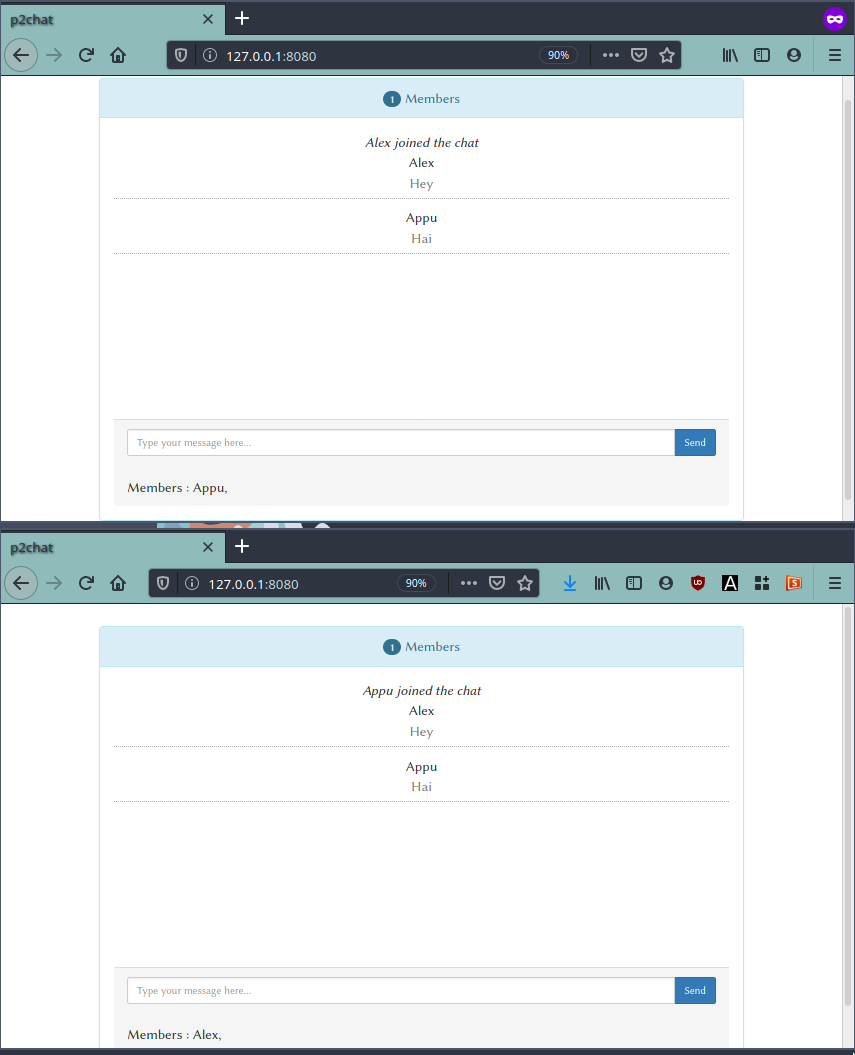
\includegraphics[scale=.4]{result.png}
		\caption{Result Chat}
		
	\end{figure}
\end{center}











\chapter{CONTRIBUTIONS}

Each member of team had contributed equally to the project. The parts that were worked on were the vue.js code, HTML and the p2p script to call the webtrackers for the webRTC. 






\chapter{CONCLUSION}

Decentralised networks can be an effective method of communication and sharing that prioritises encryption and privacy for all users. The growing number of privacy concerns due to the actions of various central powers can negated through the use of these networks, especially since they are fast and inexpensive to setup and maintain. This chatting app can enable easy communication and data sharing while also being inexpensive and safe to use for all involved users.
\newpage



\begin{thebibliography}{1}
	\bibitem{nist} Christensson, Per. "P2P Definition." TechTerms. Sharpened Productions, 2006. Web. 16 June 2020. 
	\url{https://techterms.com/definition/p2p}
	
\end{thebibliography}


\begin{appendices}
\chapter{Sample Code}
\section{App.vue}
\begin{lstlisting}[language=HTML]

<template>
<div class="container">
<div id="app" class="row">
<div class="col-xl-8 col-lg-12 col-md-6 col-sm-12 col-12">
<div class="panel panel-info">
<div class="panel-heading">
<span class="badge">{{ Object.keys(members).length }}</span> Members
</div>
<div class="panel-body">
<div v-if="joined">
<em><span v-text="status"></span></em>
<div class="chat-wrapper" ref="chatWrapper">
<ul class="chat">
<li class="left clearfix" v-for="message in messages">
<div class="chat-body clearfix">
<div class="header">
<strong class="primary-font">
{{ message.username }}
</strong>
</div>
<p>
{{ message.message }}
</p>
</div>
</li>
</ul>
</div>
<div class="panel-footer">
<div class="input-group">
<input id="btn-input" type="text" name="message" class="form-control input-sm" placeholder="Type your message here..." v-model="newMessage" ref="messageInputField" @keyup.enter="sendMessage">

<span class="input-group-btn">
<button class="btn btn-primary btn-sm" id="btn-chat" @click="sendMessage">Send</button>
</span>
</div><br/>
<div class="input-group">
Members : 
<span v-for="member in members"><b>{{ member }}</b>, </span>
</div>
</div>
</div>
<div v-else>
<div class="form-group">
<label>Room Name</label>
<input type="text" class="form-control" placeholder="chat room name" v-model="room" @keyup.enter="joinChat">
</div>
<div class="form-group">
<label>Username</label>
<input type="text" class="form-control" placeholder="enter your username to join chat" v-focus v-model="username" @keyup.enter="joinChat">
</div>
<button class="btn btn-primary" @click="joinChat">JOIN</button>
</div>
</div>
</div>
</div>
</div>
</div>
</template>

<script>
const P2PT = require('p2pt')

module.exports = {
data () {
return {
joined: false,
room: 'general',
username: '',
members: {},
newMessage: '',
messages: [],
status: ''
}
},

methods: {
init () {
this.peers = {}

let announceURLs = [
"wss://tracker.openwebtorrent.com",
"wss://tracker.sloppyta.co:443/announce",
"wss://tracker.novage.com.ua:443/announce",
"wss://tracker.btorrent.xyz:443/announce",
]
if (window.location.hostname === "localhost") {
announceURLs = ["ws://localhost:5000"]
}

this.p2pt = new P2PT(announceURLs, 'peer2chat' + this.room)
},

joinChat () {
if (this.room.trim() === '' || this.username.trim() === '') {
return
}

this.init()
this.joined = true
this.status = `${this.username} joined the chat`
this.usernames = {}

this.listen()

this.$nextTick(() => {
this.$refs.messageInputField.focus()
})
},

sendMessage () {
if (this.newMessage.trim() === '') {
return
}

const message = {
username: this.username,
message: this.newMessage
}

// Clear input field
this.newMessage = ''

for (var key in this.peers) {
this.p2pt.send(this.peers[key], JSON.stringify(message))
}

this.messages.push(message)
this.scrollDown()
},

listen () {
const $this = this
this.p2pt.on('peerconnect', (peer) => {
$this.peers[peer.id] = peer
})

this.p2pt.on('peerclose', (peer) => {
delete $this.peers[peer.id]
delete $this.members[peer.id]
})

this.p2pt.on('msg', (peer, msg) => {
msg = JSON.parse(msg)

$this.members[peer.id] = msg.username
$this.messages.push({
username: msg.username,
message: msg.message
})
$this.scrollDown()
})
this.p2pt.start()
},

scrollDown () {
this.$nextTick(() => {
var elem = this.$refs.chatWrapper
elem.scrollTop = elem.clientHeight + elem.scrollHeight
})
}
}
}
</script>

\end{lstlisting}
\newpage


\section{index.html}
\begin{lstlisting}[language=c++]


<!DOCTYPE html>
<html lang="en">
<head>
<meta charset="UTF-8">
<meta name="viewport" content="width=device-width, initial-scale=1">
<title>p2chat</title>
<link rel="stylesheet" href="//netdna.bootstrapcdn.com/bootstrap/3.3.4/css/bootstrap.min.css" async="async">
</head>
<body>
<div class="container" id="app"></div>
</body>
</html>

\end{lstlisting}


\end{appendices}


\end{document}
